%-----------------------------------------------------------------------------%
% Packages & Other Configurations
%-----------------------------------------------------------------------------%
\RequirePackage{fix-cm}  % Fix Font shape `OT1/cmr/m/n' size substitution.
\documentclass[a4paper,10pt]{article}
\usepackage[top=0.3in, bottom=0.3in, left=1in, right=0.9in]{geometry}
\usepackage[utf8]{inputenc} %add acents
\usepackage{setspace} % command \doublespacing etc...
\usepackage{lineno} % number lines
\usepackage{epsf,epsfig} % includegraphics [pdf, png etc]
\usepackage{amsmath} %adicionei esse pacote pra vc poder usar o draft%
\usepackage{textcomp} %símbolos de texto
\usepackage{natbib} % bibtex - adicionar referencia
% \usepackage{url} % for bibtex - configuracoes de urls
\usepackage{tabularx} % for tables
\usepackage[hidelinks]{hyperref}  % Add URL links.
% \usepackage[bookmarks=false,colorlinks=true,urlcolor={green},linkcolor={green},pdfstartview={XYZ null null 1.22}]{hyperref} %all references
\usepackage{tikz}
\usepackage{lscape}
\usepackage{siunitx}
\usepackage{geometry}

%-----------------------------------------------------------------------------%
% Adicionar a Watermark
%-----------------------------------------------------------------------------%
\usepackage{draftwatermark}
\SetWatermarkAngle{45}
\SetWatermarkLightness{0.9}
\SetWatermarkFontSize{5cm}
\SetWatermarkScale{0.3}
\SetWatermarkText{Exercícios 3 - Oceanografia}
%-----------------------------------------------------------------------------%
% Informações sobre o PDF
%-----------------------------------------------------------------------------%
\pdfinfo{%
  /Title    (GEO232 - Exercícios 3)
  /Author   (Ju Leonel)
  /Creator  (Ju Leonel)
  /Producer (Ju Leonel)
  /Subject  (Intro oceanografias)
  /Keywords (Intro oceanografia, Exercícios 3)}

%-----------------------------------------------------------------------------%
% Documento
%-----------------------------------------------------------------------------%
\title{GEO232 - Introdução à Oceanografia - Exercícios 3}
\author{\vspace{-10ex}}
\date{\vspace{-10ex}}

\geometry{hmargin=1cm,vmargin=1cm}

\begin{document}
 \maketitle
 \phantom{}



1. Abaixo encontram-se dados de temperatura e salinidade de uma estação oceanográfica no Oceano Atlântico em 20\textdegree N e as médias de temperatura e salinidade para diferentes profundidades no Atlântico Sul. 

\begin{center}
  \begin{tabular}{|c|c|c|c|c|c|}
    \hline
    \multicolumn{3}{|c|}{Atlântico Norte} & \multicolumn{3}{|c|}{Atlântico Sul} \\ \hline
   Profundidade    & Temperatura    & Salinidade & Profundidade    & Salinidade    & Temperatura\\ \hline          
    (m)     & (\textcelsius) & (\textperthousand) & (m)  & (\textperthousand) & (\textcelsius)    \\
    100     & 16.0           & 36.1               & 0    & 35.2           &  12.7          \\
    200     & 13.0           & 35.7               & 20   & 35.3           &  12.6          \\
    400     & 11.0           & 35.4               & 50   & 35.3           &  12.1          \\
    500     & 9.0            & 35.3               & 100  & 35.3           &  11.5          \\
    600     & 8.0            & 35.2               & 150  & 35.2           &  10.3          \\
    850     & 11.8           & 36.9               & 250  & 34.9           &  8.3           \\
    950     & 11.2           & 36.6               & 400  & 34.7           &  6.4           \\
    1200    & 9.9            & 36.3               & 600  & 34.5           &  4.2           \\
    2000    & 4.0            & 35.0               & 800  & 34.5           &  3.0           \\
    2200    & 3.5            & 34.9               & 1000 & 34.5           &  2.5           \\    
    2500    & 2.0            & 34.8               & 1200 & 34.6           &  2.3           \\    
    3000    & 0.0            & 34.7               & 1400 & 34.7           &  2.2           \\    
    4000    & -1.2           & 34.6               & 1750 & 34.8           &  1.9           \\     
    5000    & -1.9           & 34.5               & 2500 & 34.8           &  1.5           \\    
    -       & -              & -                  & 3500 & 34.8           &  1.5           \\  
    -       & -              & -                  & 4500 & 34.8           &  0.9           \\ 
    -       & -              & -                  & 4500 & 34.7           &  0.1           \\
    \hline
  \end{tabular}
\end{center}

\begin{itemize}
  \item[(a)] Grafique os dados no diagrama T-S de acordo com temperatura e salinidade da tabela acima. Faça um diagrama para os dados do Atlântico Norte e outro para o Atlântico Sul.
  \item[(b)] Desenhe uma linha conectando os pontos em ordem crescente de profundidade.
  \item[(c)] Usando as informações da tabela abaixo identifique e nomeie as  massas d'água que aparecem nesse diagrama em cada um dos oceanos.
  \item[(d)] Faça uma consulta bibliográfica e encontre os intervalos de temperatura e salinidade para cada uma das massas d'água citadas na tabela. Não esqueça de citar as referências bibliográficas utilizadas. 
  \end{itemize}

\begin{center}
  \begin{tabular}{|c|c|p{6cm}|}
    \hline
        \multicolumn{3}{|c|}{Massas d'água do Atlântico Norte} \\
    \hline          
    Massa d'água                       & Origem & Características    \\ \hline
    Água Antártica de Fundo (AFA)      & Mar de Weddell        & Água de fundo com temperaturas mínimas \\ \hline
    Água Profunda do Atlântico Norte (APAN)   & Próximo a Groelândia  & Salinidade máximas intermediária, pode apresentar temperatura máxima intermediária, rica em oxigênio \\ \hline
    Água superficial                   & Regional              & Variável, geralmente quente \\ \hline
    Água Intermediária do Mediterrâneo (AIM) & Mediterrâneo          & Altas salinidades e temperaturas mais altas em profundidades intermediárias \\ \hline
    \multicolumn{3}{|c|}{Massas d'água do Atlântico Sul} \\ \hline
    Água Intermediária Antártica (AIA)      & Convergência Antártica   & Baixas salinidades e temperaturas mais baixas em profundidades intermediárias \\ \hline
     Água Profunda do Atlântico Norte (APAN)   & Próximo a Groelândia  & Salinidade máximas intermediária, pode apresentar temperatura máxima intermediária, rica em oxigênio \\ \hline
     Água Central do Atlântico Sul (ACAS)  & Centro do Giro Subtropical  & Altas temperaturas e salinidades \\ 
    \hline
  \end{tabular}
\end{center}  
  
  
  
  
  
\def\width{8}
\def\hauteur{10}

\begin{center}
  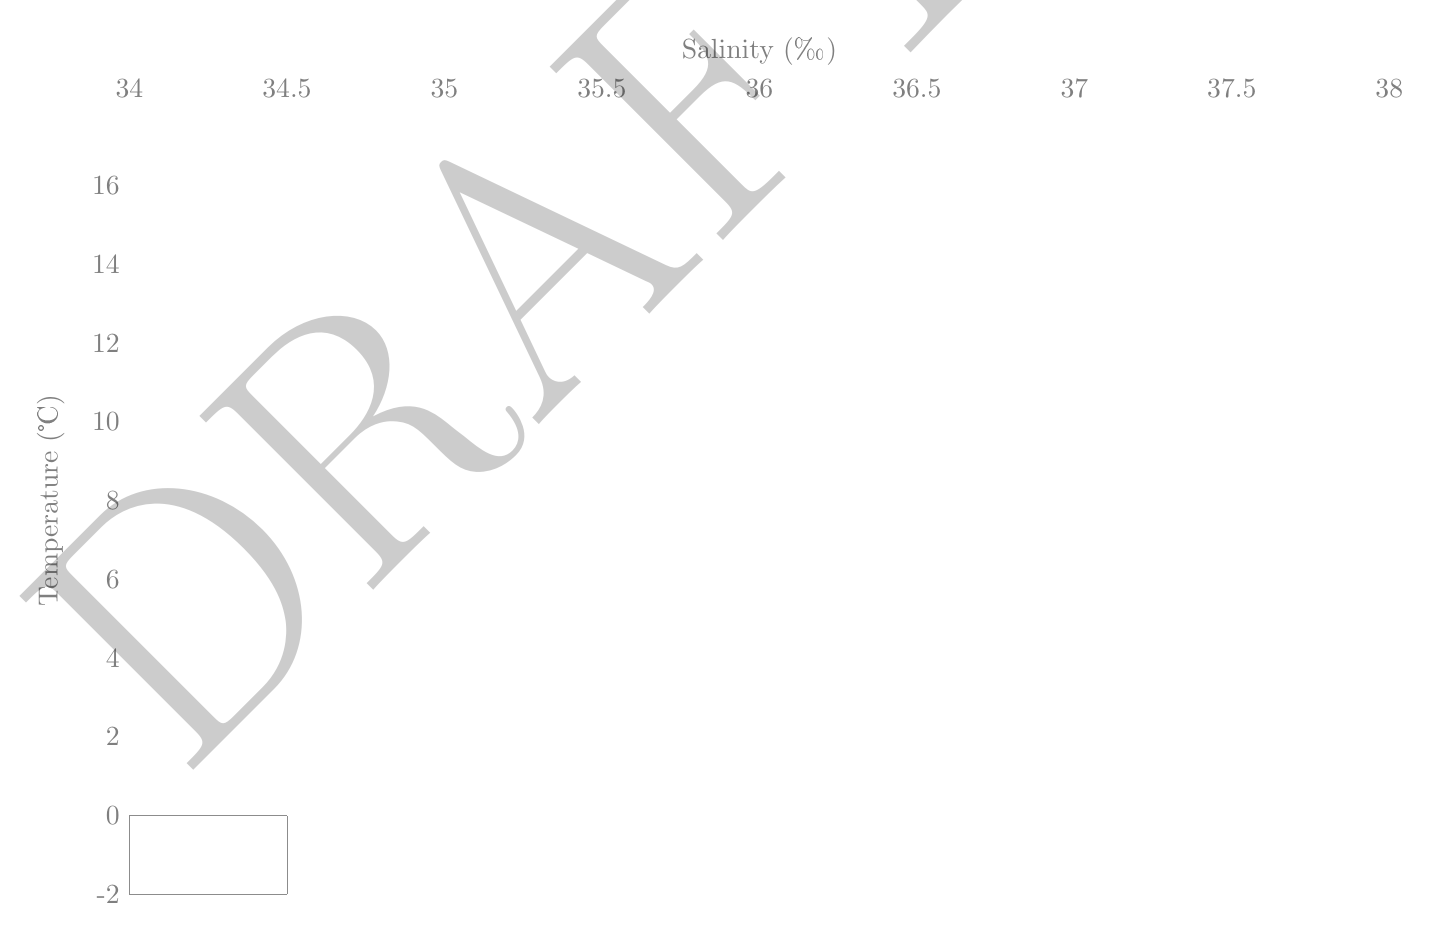
\begin{tikzpicture}[x=2cm, y=1cm, semitransparent]
  % Grid.
  \draw[xstep=2cm, ystep=1cm, line width=0.1mm, black!90!white] (0,0) grid (\width,\hauteur);
  % x-tickslabels.
  \draw[black] ( 0, 10) node[anchor=south] {34};
  \draw[black] ( 1, 10) node[anchor=south] {34.5};
  \draw[black] ( 2, 10) node[anchor=south] {35};
  \draw[black] ( 3, 10) node[anchor=south] {35.5};
  \draw[black] ( 4, 10) node[anchor=south] {36};
  \draw[black] ( 5, 10) node[anchor=south] {36.5};
  \draw[black] ( 6, 10) node[anchor=south] {37};
  \draw[black] ( 7, 10) node[anchor=south] {37.5};
  \draw[black] ( 8, 10) node[anchor=south] {38};
  % x-labels.
  \draw[black] (4, 11) node[anchor=north] {Salinity (\textperthousand)};
  % y-labels.
  \draw[black] (-0.5, 5) node[rotate=90] {Temperature (\textcelsius)};
  % y-tickslabels left.
  \draw[black] (0,  9) node[anchor=east] {16};
  \draw[black] (0,  8) node[anchor=east] {14};
  \draw[black] (0,  7) node[anchor=east] {12};
  \draw[black] (0,  6) node[anchor=east] {10};
  \draw[black] (0,  5) node[anchor=east] { 8};
  \draw[black] (0,  4) node[anchor=east] { 6};
  \draw[black] (0,  3) node[anchor=east] { 4};
  \draw[black] (0,  2) node[anchor=east] { 2};
  \draw[black] (0,  1) node[anchor=east] { 0};
  \draw[black] (0,  0) node[anchor=east] {-2};
  \end{tikzpicture}
\end{center}


\def\width{8}
\def\hauteur{10}

\begin{center}
  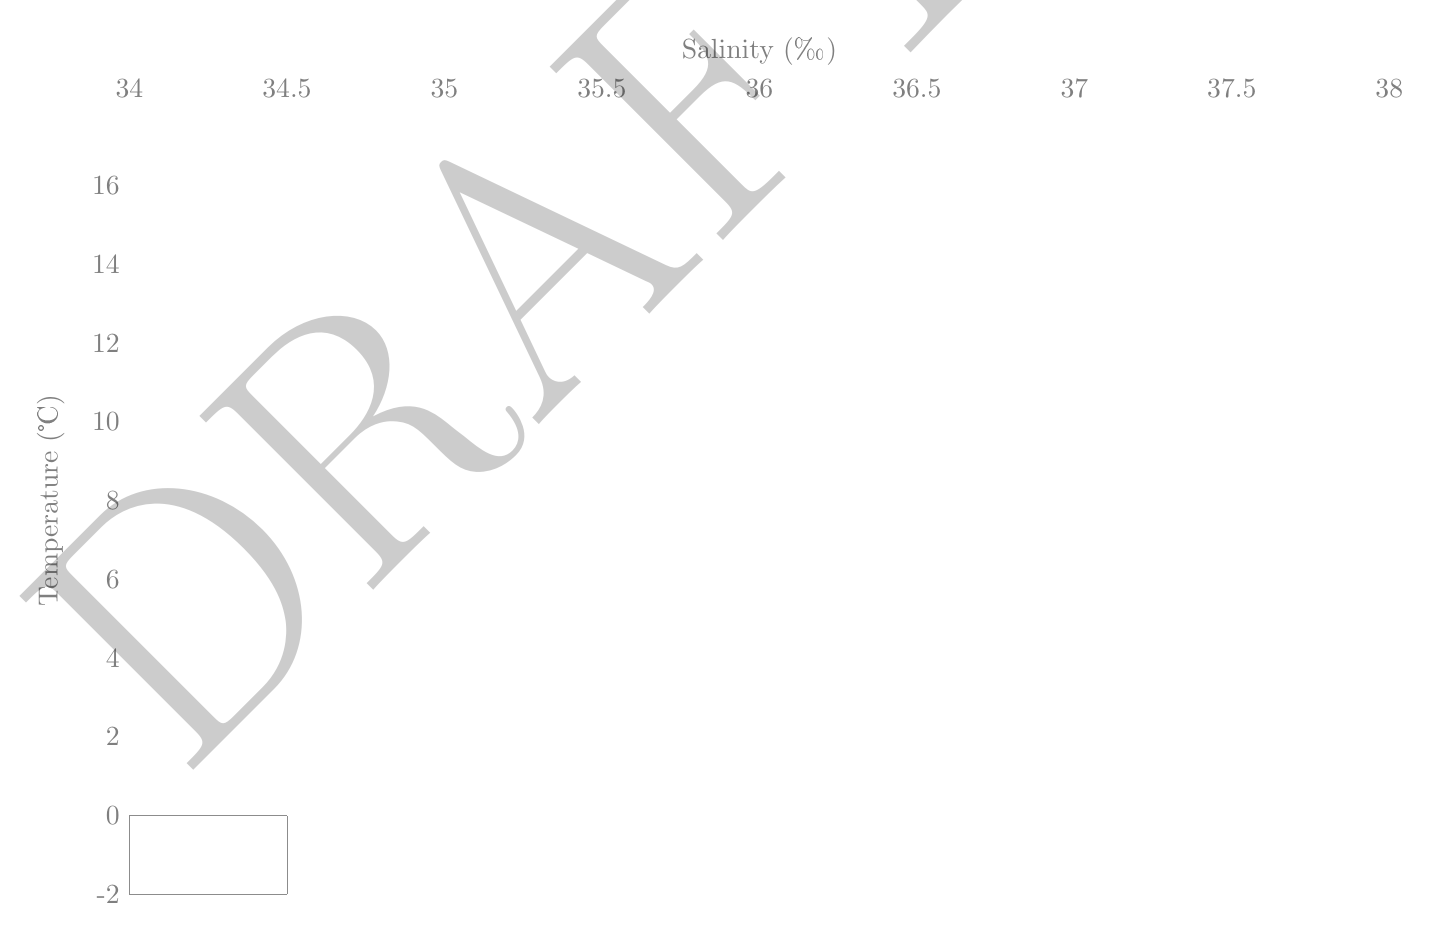
\begin{tikzpicture}[x=2cm, y=1cm, semitransparent]
  % Grid.
  \draw[xstep=2cm, ystep=1cm, line width=0.1mm, black!90!white] (0,0) grid (\width,\hauteur);
  % x-tickslabels.
  \draw[black] ( 0, 10) node[anchor=south] {34};
  \draw[black] ( 1, 10) node[anchor=south] {34.5};
  \draw[black] ( 2, 10) node[anchor=south] {35};
  \draw[black] ( 3, 10) node[anchor=south] {35.5};
  \draw[black] ( 4, 10) node[anchor=south] {36};
  \draw[black] ( 5, 10) node[anchor=south] {36.5};
  \draw[black] ( 6, 10) node[anchor=south] {37};
  \draw[black] ( 7, 10) node[anchor=south] {37.5};
  \draw[black] ( 8, 10) node[anchor=south] {38};
  % x-labels.
  \draw[black] (4, 11) node[anchor=north] {Salinity (\textperthousand)};
  % y-labels.
  \draw[black] (-0.5, 5) node[rotate=90] {Temperature (\textcelsius)};
  % y-tickslabels left.
  \draw[black] (0,  9) node[anchor=east] {16};
  \draw[black] (0,  8) node[anchor=east] {14};
  \draw[black] (0,  7) node[anchor=east] {12};
  \draw[black] (0,  6) node[anchor=east] {10};
  \draw[black] (0,  5) node[anchor=east] { 8};
  \draw[black] (0,  4) node[anchor=east] { 6};
  \draw[black] (0,  3) node[anchor=east] { 4};
  \draw[black] (0,  2) node[anchor=east] { 2};
  \draw[black] (0,  1) node[anchor=east] { 0};
  \draw[black] (0,  0) node[anchor=east] {-2};
  \end{tikzpicture}
\end{center}


\end{document}
